\documentclass[11pt]{article}

\usepackage{graphicx}
\usepackage{fullpage}
\usepackage{hyperref}
\usepackage{xcolor}
%\usepackage{times} % this gave me errors, didn't let me use \tt
\usepackage{amsfonts,amsthm,amsmath}
\usepackage{algorithm,algorithmic,xspace,hyperref}
\usepackage{tikz}
\usetikzlibrary{arrows}
    
%\textwidth 7in
%\textheight 9.5in

\pdfpagewidth 8.5in
\pdfpageheight 11in 




% Margins are default 1in. on all sides
% thus, if you wanted .5 on the left, and right
% you'd do \oddsidemargin -.25in.
% \evensidemargin -.25in. and
% \textwidth 7in.
%\oddsidemargin 0in
%\evensidemargin 0in


\newtheorem{claim}{Claim}
\newtheorem{definition}{Definition}
\newtheorem{theorem}{Theorem}
\newtheorem{lemma}{Lemma}
\newtheorem{observation}{Observation}

\newtheorem{problem}{Problem}



\begin{document}

\begin{center}
\Large{\textbf{CS 123 -- Doubling Edge Weights}}\\
\Large{deadline: Tuesday, December 3 at 11:59 pm}
\end{center}

Description of your assignment
\subsection*{Submission Format}

On Gradescope submit {\tt submission.py}  (the name must match exactly)  containing your solution.
It will be called as follows: 

\begin{verbatim}
	python3 submission.py input_file output_file
\end{verbatim}
\section{Implementing the Double Edge Weights Algorithm}

In this exercise you will implement $doubleEdgeWeights()$ function.

\subsection*{Input}

For both parts of the assignment, the input is a text file with the following format: 

We have uploaded files corresponding to the visible test cases on Gradescope.
They may help you test and debug locally.
Passing these test cases does not guarantee your code is correct!

Here is an image of a graph:

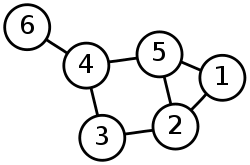
\includegraphics{images/graph.png}

\subsection*{Output}

\subsection*{Starter Code}

\subsection*{Tips}

\subsection*{Example}

\end{document}

